\documentclass[aspectratio=1610]{beamer}
\usepackage[T1]{fontenc}
\usepackage[utf8]{inputenc}
\usepackage{biolinum}
\usepackage{microtype}
\usefonttheme[onlymath]{serif}
\usetheme[nofirafonts]{focus}

\usepackage[backend=bibtex,sorting=none]{biblatex}
\addbibresource{reference.bib} %BibTeX数据文件及位置
\setbeamerfont{footnote}{size=\tiny}
\usepackage{multirow}
\usepackage{booktabs}
\usepackage{color}
\usepackage{threeparttable}
\usepackage{overpic}


%% Prevents numbering on continued frames (messes up impa logo otherwise)
\setbeamertemplate{frametitle continuation}{}
\setbeamertemplate{caption}[numbered]

%% Two different options for bottom bar. Default is progressbar.
%\usetheme[nofirafonts,numbering=fullbar]{focus}
%\usetheme[nofirafonts,numbering=none]{focus}

%% Leave one uncommented to choose which official IMPA color to use:
% IMPA Azul:
%\definecolor{main}{RGB}{0, 75, 135}
\definecolor{main}{RGB}{16, 52, 98}
% IMPA Cinza
%\definecolor{main}{RGB}{83, 86, 90}

%% Defines command that adds small IMPA logo to titlebars
\newcommand{\UoN}
  {\hfill {
\includegraphics[height=0.8cm]{nott_logo/nott_logo_white.png}}}

%% Sets footnote references to numeric.
\renewcommand{\thempfootnote}{\arabic{mpfootnote}}

%% Defines progressive outline for sections
\AtBeginSection[]
{
  \begin{frame}<beamer>[noframenumbering]
%    \frametitle{Outline for section \thesection}
    \frametitle{Presentation Outline \UoN}
    \tableofcontents[currentsection,hideothersubsections]
  \end{frame}
}
     
%% Suppresses outline frames for subsections.
\AtBeginSubsection[]

%% Defines Title Page.

\title{Ensemble Framework with Fuzzy Methods\\}
\subtitle{\textit{Chapter 5 of the PhD Thesis}}
\author{Zixiao Shen
	\footnote{\label{1} Intelligent Modelling and Analysis Group, School of Computer Science}
	\footnote{\label{2} Lab for Uncertainty in Data and Decision Making (LUCID)}
	\footnote{\label{3} University of Nottingham, Nottingham, NG8 1BB, United Kingdom}}
\titlegraphic{\vspace*{2em}
              
\includegraphics[scale=0.25]
                {nott_logo/UoN_logo.png}}
\institute{Presented by:\\ 
            Zixiao Shen\\
            2$^\text{nd}$ Oct 2020}
\date{\textit{\tiny{\url{}}}}

%https://arxiv.org/pdf/2005.09856.pdf

\begin{document}

\begin{frame}
  \titlepage
\end{frame}

\section{Introduction}

\begin{frame}
\frametitle{What is Feature Selection (FS) ? \UoN}

\textbf{Feature selection (FS)} is the process of selecting of relevant features for use in model construction. 

	\begin{figure}
		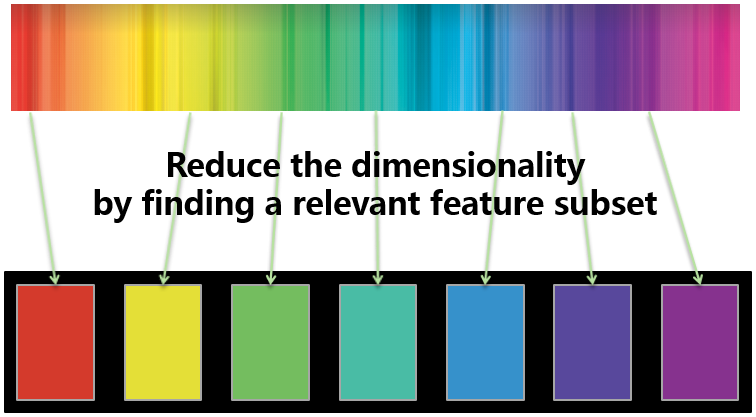
\includegraphics[scale=0.6]{Figures/Feature_Selection.png}
%		\caption{\scriptsize{Framework of Feature Selection}}
	\end{figure}

\end{frame}



\begin{frame}
\frametitle{Main Issues \UoN}
	There exist plenty of different feature selection (FS) methods

	\begin{figure}
	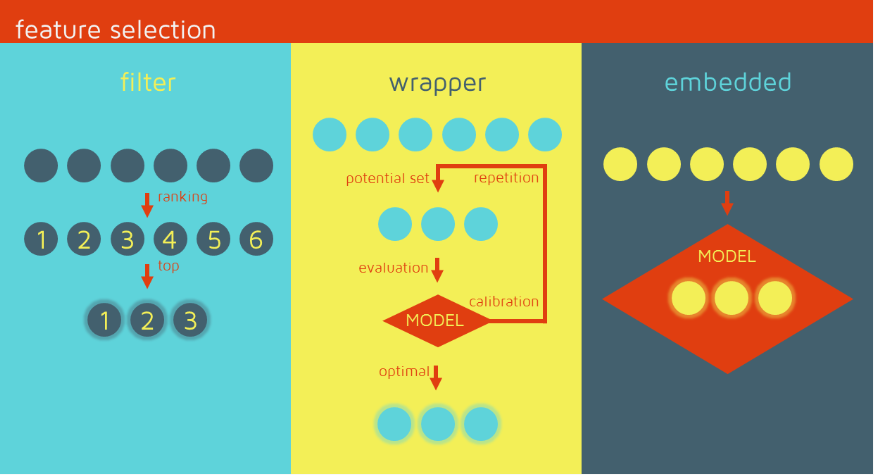
\includegraphics[scale=0.4]{Figures/FS_Methods.png}
	%		\caption{\scriptsize{Framework of Feature Selection}}
	\end{figure}

	\begin{itemize}
		\item The performance of the various FS methods is data dependent;
		\item It's not possible to state categorically the optimal FS method for all kinds of data.
	\end{itemize}
\end{frame}


\begin{frame}
\frametitle{Possible Solutions \UoN}

\begin{enumerate}
	\item Combination methods using the diversity kinds of FS algorithms~\footfullcite{shen2019novel};
	\item Use meta-learning method to choose the best algorithm for a given dataset.
\end{enumerate}

\begin{columns}
	\begin{column}{0.5\textwidth}
		\begin{figure}
			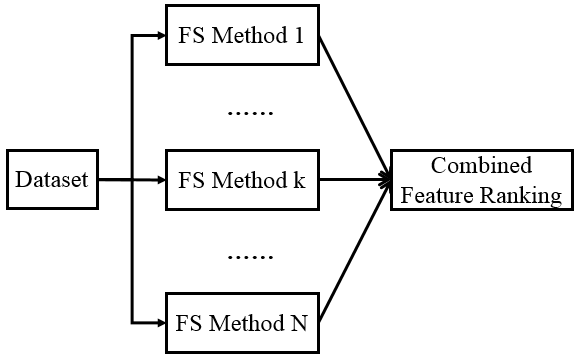
\includegraphics[scale=0.4]{Figures/Combined_FS.png}
			\caption{\scriptsize{Combined approach for FS}}
		\end{figure}
	\end{column}

	\begin{column}{0.5\textwidth}
		\begin{figure}
			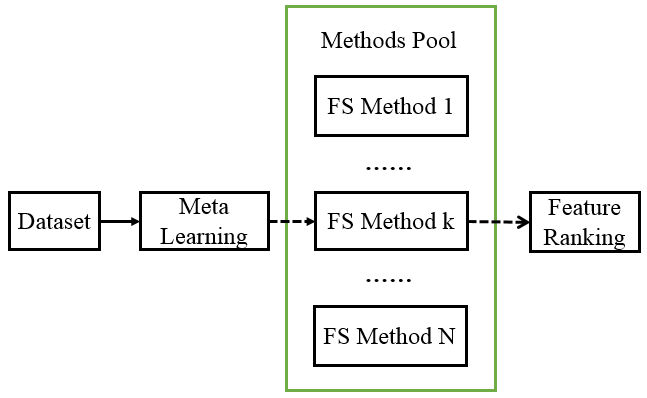
\includegraphics[scale=0.4]{Figures/Meta_FS.png}
			\caption{\scriptsize{Meta Learning approach for FS}}
		\end{figure}
	\end{column}

\end{columns}
\end{frame}



\section{Literature Review}
\begin{frame}
\frametitle{Literature Review \UoN}
	\begin{block}{Homogeneous approach (Data variation approach)}
		\begin{itemize}
			\item The same FS method using different training data are implemented on the different nodes distributed by the dataset.
		\end{itemize}
	\end{block}
		
	\begin{block}{Heterogeneous approach (Function variation approach)}
		\begin{itemize}
			\item Different FS methods are applied on the same training dataset.
		\end{itemize}
	\end{block}
\end{frame}


\section{Methodology}
\subsection{Overall Framework}

\begin{frame}
\frametitle{Overall Framework \UoN}
	\begin{figure}
    	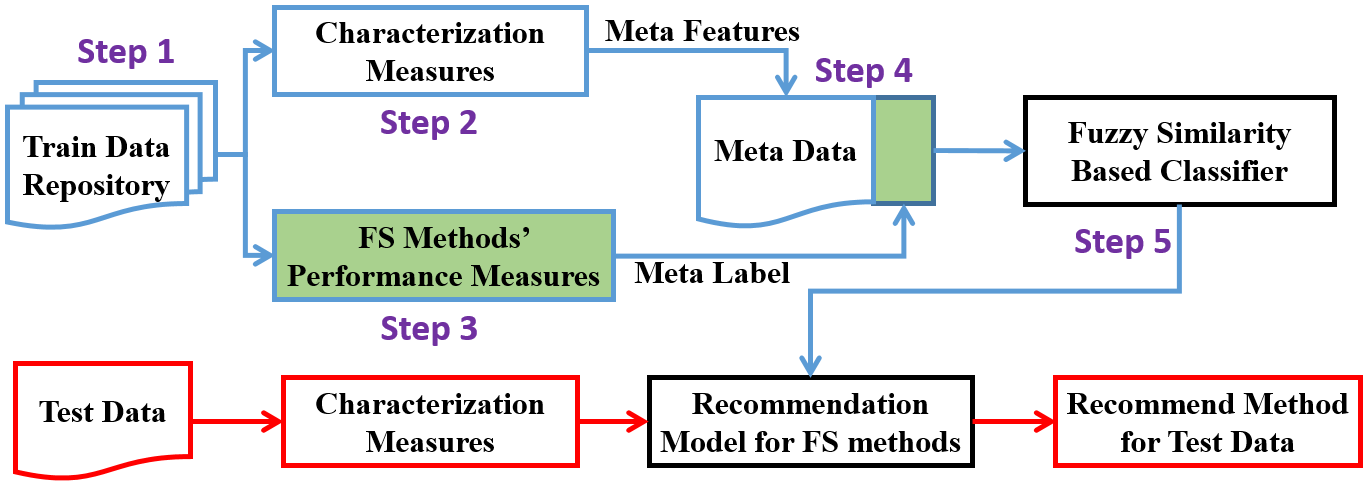
\includegraphics[scale=0.33]{Figures/Overall_Framework_step.png}
    	\caption{\scriptsize{Overall framework of the proposed architecture}}
    \end{figure}

  	\begin{enumerate}
  		\item Generation of a data repository for training;
  		\item Meta features extraction;
  		\item FS methods' performance measures;
  		\item Meta data construction;
  		\item Recommendation using fuzzy similarity measure.
  	\end{enumerate}
\end{frame}

\subsection{Generation of a Data Repository for Training}
\begin{frame}
\frametitle{Generation of a Data Repository for Training \UoN}

\begin{columns}
	\begin{column}{0.5\textwidth}
	\begin{itemize}
		\item Construct a data repository that covers a variety of characteristics using data synthesis;
		\item Madelon datasets are used on account of its high flexibility and variability;
	\end{itemize}	
	\end{column}
	
	\begin{column}{0.5\textwidth}
		\begin{figure}
			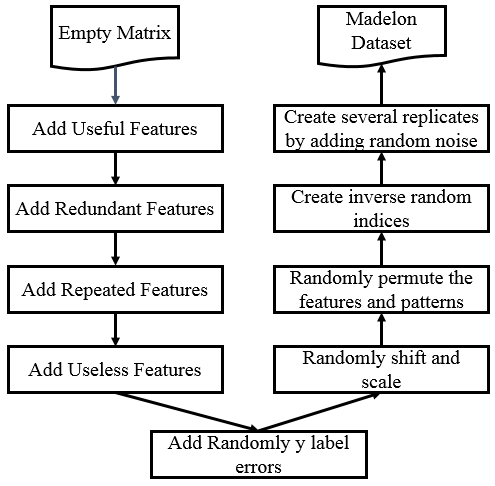
\includegraphics[scale=0.5]{Figures/Madelon.png}
		\caption{\scriptsize{Generation Process of Madelon Dataset}}
		\end{figure}
	\end{column}
\end{columns}
\end{frame}



\begin{frame}
\frametitle{Generation of a Data Repository for Training \UoN}
	\begin{itemize}
		\item Different kinds of madelon datasets are generated by varying 11 different parameters.
	\end{itemize}	
	
	\begin{table}[tb]\scriptsize
		\caption{\scriptsize{Parameters for data synthesis using Madelon dataset}}
		\centering
		\begin{tabular}{c|c|c}
			\hline
			\textbf{Alias}  & \textbf{Meaning}   & \textbf{Value Range}  \\ \hline
			P1  & Number of Classes  &   2  \\ \hline
			P2  & \begin{tabular}[c]{@{}c@{}}Number of Useful Features\\ \textit{(initially drawn to explain the concept)}\end{tabular}  
			& [4, 5,..., 20] \\ \hline
			P3  & \begin{tabular}[c]{@{}c@{}}Number of Redundant Features\\ \textit{(linearly dependent upon the useful features)}\end{tabular}  
			& [0, 1,..., 20] \\ \hline
			P4  & \begin{tabular}[c]{@{}c@{}} Number of Repeated Features\\ \textit{(repeating P2 and P3 at random)}\end{tabular}    
			& [0, 1,..., 20] \\ \hline
			P5  & \begin{tabular}[c]{@{}c@{}} Number of Useless Features\\ \textit{(Drawn at random regardless of class label)}\end{tabular}
			& [0, 1,..., 20] \\ \hline
			P6  & Number of Samples per Cluster & [10, 11,..., 70] \\ \hline
			P7  & Number of Cluster per Class  & [2, 3,..., 7] \\ \hline
			P8  & Random Seed       & [1, 2,..., 1000]   \\ \hline
			P9  & Factor multiplying the hypercube dimension  & [2, 3,..., 10]  \\ \hline
			P10 & Fraction of y labels to be randomly exchanged & [0.01, 0.02, ..., 0.1] \\ \hline
			P11 & Flag to enable or disable random permutations & [0, 1] \\ \hline
		\end{tabular}
	\end{table}
\end{frame}


\subsection{Meta Feature Extraction}
\begin{frame}
\frametitle{Meta Feature Extraction \UoN}
	\begin{itemize}
		\item To learn meta features from the synthetic dataset, we extract a set of meta features from $M$ different datasets $D_i$, $i=1,..., M$, each with the number of $S_i$ data samples ($E_1, E_2,..., E_{S_i}$) and $N_i$ features ($F_1, F_2,..., F_{N_i}$). The label information is represented using class $C$ ($c_1, c_2,..., c_{S_i}$) for different data samples.
	\end{itemize}
	
	
	\begin{columns}
		\begin{column}{0.5\textwidth}
			\begin{enumerate}
				\item[1.] Number of Samples (NS)
				\item[3.] Avg. Asymmetry of Features (AAF)
				\begin{equation}\footnotesize %\nonumber
%					AAF(D_i) =  
					\frac{3}{N_i} \sum^{N_i}_{j=1} \frac{Mean(F_j) - Med.(F_j)}{Std(F_j)}
				\end{equation}
				\item[5.] Avg. Coef. of Var. of Features (ACVF)
				\begin{equation}\footnotesize
%					ACVF(D_i) = 
				\frac{1}{N_i} \sum^{N_i}_{j=1} \frac{Std(F_j)}{Mean(F_j)}
				\end{equation}
			\end{enumerate}
		\end{column}
		
		\begin{column}{0.5\textwidth}
			\begin{enumerate}
				\item[2.] Number of Features (NF)
				\item[4.] Avg. Correlation of Features (ACF)
				\begin{equation}\footnotesize %\nonumber
%				ACF(D_i) = 
				\frac{2}{N_i(N_i-1)} \sum^{N_i-1}_{j=1} \sum^{N_i}_{k=j+1} Pearson(F_j, F_k)
				\end{equation}
				\item[6.] Avg. Entropy of Features (AEF)
				\begin{equation}\footnotesize
%				AEF(D_i) = 
				\frac{1}{N_i} \sum^{S_i}_{k=1}Entropy(F_j)
				\end{equation}
			\end{enumerate}
		\end{column}
	\end{columns}
\end{frame}

\subsection{Performance Measures of FS Methods}
\begin{frame}
\frametitle{Performance Measures of FS Methods \UoN}
The best FS method for a given synthetic dataset has been generated as the label.

	\begin{columns}
		\begin{column}{0.5\textwidth}
			\begin{figure}
				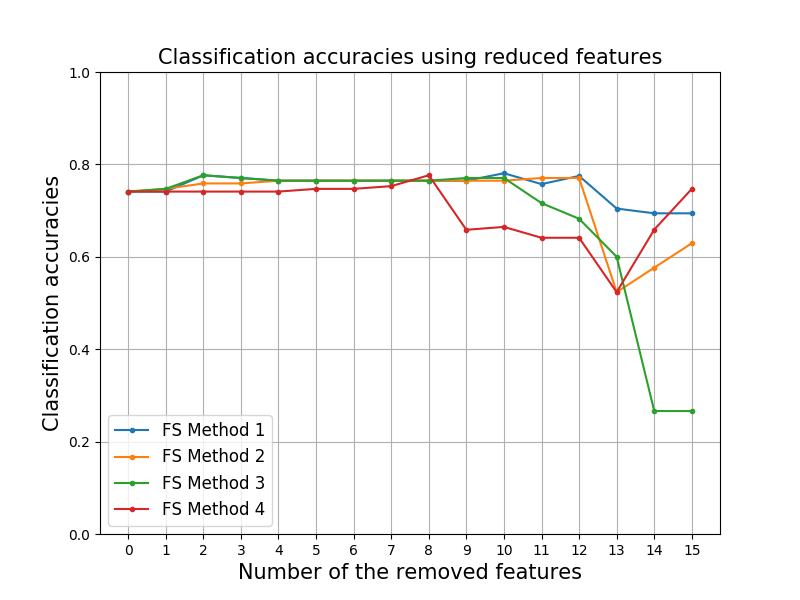
\includegraphics[scale=0.3]{Figures/Accuracy.png}
				\caption{\scriptsize{Demonstration of classification accuracies using reduced features}}
			\end{figure}
		\end{column}

		\begin{column}{0.5\textwidth}
			\begin{enumerate}
				\item Divide the data using 10-fold CV;
				\item Implement the candidate FS method to rank the features using the training set;
				\item Model the classifier using the training set and make the prediction on the test set;
				\item Calculate mean classification accuracy across different folds.
			\end{enumerate}
		
		Weighted sum (WS) of the accuracies:
			\begin{equation}\nonumber
			WS = \sum Acc. * \% RemovedFeatures
			\end{equation}
		\end{column}
	\end{columns}
\end{frame}


\subsection{Meta Data Construction}
\begin{frame}
\frametitle{Meta Data Construction \UoN}
\begin{itemize}
	\item The FS method with the highest WS value is selected as the meta label for the dataset;
	\item The meta data is constructed by combining the six different meta features $MF_p$, $(1 \leq p \leq 6)$ and the corresponding meta label for each dataset $D_i$.
\end{itemize}

\begin{table}[h]\footnotesize
	\caption{\scriptsize{Demonstration of Meta Data}}
	\centering
	\begin{tabular}{|c|c|c|c|c|c|c|c|}
		\hline
		\multirow{2}{*}{\textbf{Data}} & \multicolumn{6}{c|}{\textbf{Meta Features}} & \multirow{2}{*}{\begin{tabular}[c]{@{}c@{}}\textbf{Meta}\\ \textbf{Target}\end{tabular}} \\ \cline{2-7}
		& $MF_1$   & $MF_2$  & ... & $MF_p$  & ... & $MF_{6}$ &   \\ \hline
		$D_1$   & $w_{1,1}$  & $w_{1,2}$ & ... & $w_{1,p}$ & ... & $w_{1, 6}$ &  $Opt_1$  \\ \hline
		$D_2$   & $w_{2,1}$  & $w_{2,1}$ & ... & $w_{2,p}$ & ... & $w_{2, 6}$ &  $Opt_2$     \\ \hline
		…                     & …    & …   & …   & …   & …   & …   & …                  \\ \hline
		$D_i$   & $w_{i,1}$  & $w_{i,1}$ & ... & $w_{i,p}$ & ... & $w_{i, 6}$ & $Opt_i$     \\ \hline
		…                     & …    & …   & …   & …   & …   & …   & …                  \\ \hline
		$D_M$   & $w_{M,1}$  & $w_{M,1}$ & ... & $w_{M,p}$ & ... & $w_{M, 6}$ & $Opt_M$     \\ \hline
	\end{tabular}
\end{table}
\end{frame}

\subsection{Recommendation using Fuzzy Similarity Measure}
\begin{frame}
\frametitle{Recommendation using Fuzzy Similarity Measure \UoN}
\begin{columns}
	\begin{column}{0.5\textwidth}
		\begin{itemize}\footnotesize
			\item Blue line shows data flow for training process;
			\item Red line shows data flow for testing process.
		\end{itemize}
		
		\begin{figure}
			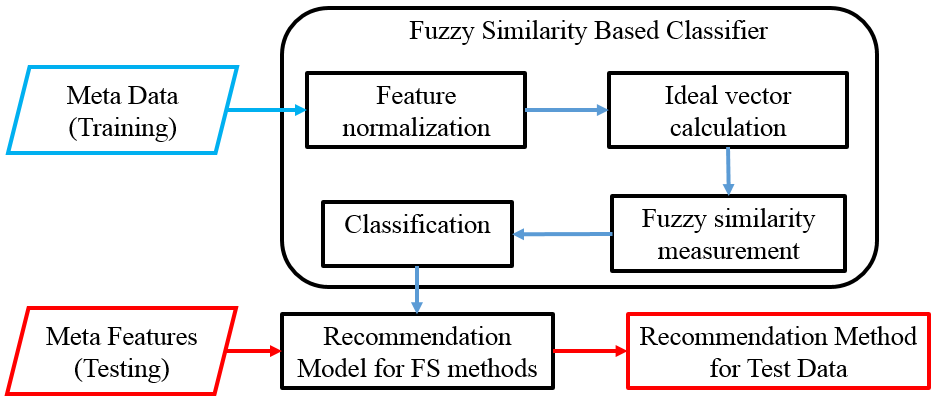
\includegraphics[scale=0.3]{Figures/Similarity_Classifier.png}
			\caption{\scriptsize{Framework of fuzzy similarity classifer}}
		\end{figure}
	\end{column}

	\begin{column}{0.5\textwidth}
		\begin{enumerate}\scriptsize
			\item For the training set, standardize each feature using the Z-score normalization process;
			\item Calculate the ideal vector $\vec{v}_l$ for the $l^{th}$ class using geometric mean;
			\begin{equation}\nonumber
			\vec{v}_l(p) = \sqrt[Z_l]{\prod_{q=1}^{Z_l}\vec{x_q}(p)}, \  1 \leq p \leq 6
			\end{equation}
			\item Apply the same standardization process to the meta features extracted from the test dataset;	
			\item Implement a similarity measurement in the form of generalized \L ukasiewicz algebra. Combine the similarity measures from different features using geometric mean;
			\begin{equation}\label{eqGeo}
			S \langle \vec{y_r}, \vec{v}_l \rangle = \sqrt[6]{\prod_{p=1}^{6} \sqrt{1 - |\vec{y_r}(p)^2- \vec{v}_l(p)^2|}}
			\end{equation}
			\item Classify test datasets into the class of corresponding ideal vector with the highest fuzzy similarity value.
		\end{enumerate}
	\end{column}
\end{columns}
\end{frame}

  
\section{Experiments \& Results}
\subsection{Datasets}
\begin{frame}
\frametitle{Datasets \UoN}

\begin{columns}[T]
	\begin{column}{0.5\textwidth}
		\begin{block}{Training Data Repository}
			\begin{itemize}
				\item[$\blacktriangleright$] 1000 datasets were generated by using randomly selected parameter values.
			\end{itemize}
		\end{block}
	
		\begin{table}\tiny
		\caption{\scriptsize{Parameters for data synthesis on Madelon dataset}}
		\centering
		\begin{tabular}{c|c|c}
			\hline
			\textbf{Alias}  & \textbf{Meaning}   & \textbf{Value Range}  \\ \hline
			P1  & Number of Classes  &   2  \\ \hline
			P2  & Number of Useful Features	& [4, 5,..., 20] \\ \hline
			P3  & Number of Redundant Features & [0, 1,..., 20] \\ \hline
			P4  & Number of Repeated Features	& [0, 1,..., 20] \\ \hline
			P5  & Number of Useless Features      & [0, 1,..., 20] \\ \hline
			P6  & Number of Samples per Cluster & [10, 11,..., 70] \\ \hline
			P7  & Number of Cluster per Class  & [2, 3,..., 7] \\ \hline
			P8  & Random Seed       & [1, 2,..., 1000]   \\ \hline
			P9  & Factor multiplying the hypercube dimension  & [2, 3,..., 10]  \\ \hline
			P10 & Fraction of y labels to be randomly exchanged & [0.01, 0.02, ..., 0.1] \\ \hline
			P11 & Flag to enable or disable random permutations & [0, 1] \\ \hline
		\end{tabular}
	\end{table}	
	\end{column}

	\begin{column}{0.5\textwidth}
		\begin{block}{Testing Data Repository}
			\begin{itemize}
				\item[$\blacktriangleright$] 8 binary classification datasets from UCI machine learning repository.
			\end{itemize}
		\end{block}
		
		\begin{table}\tiny
			\caption{\scriptsize{Description of the biomedical datasets for testing}}
			\centering
			\begin{tabular}{c c c c c}
				\toprule
				\textbf{Dataset} & \textbf{\#Fea.} & \textbf{\#Samples} & \textbf{Distribution Over Class}  \\
				\midrule
				\centering
				Appendicitis  &  7 &  106  &  85 / 21     \\
				PIMA 		  &  8 &  768  &  500 / 268   \\
				WBC			  &  9 &  699  &  458 / 241   \\
				Statlog Heart & 13 &  270  &  150 / 120   \\
				Parkinsons	  & 22 &  195  &  48 / 147    \\
				WDBC          & 30 &  569  &  212 / 357   \\
				Spectfheart   & 44 &  267  &  55 / 212    \\
				Sonar         & 60 &  208  &  97 / 111    \\
				\bottomrule
			\end{tabular}
		\end{table}
	\end{column}
\end{columns}
\end{frame}


\subsection{Feature Selection Methods}
\begin{frame}
\frametitle{Feature Selection Methods \UoN}
	\begin{itemize}
		\item Four filter FS methods which come from different categories were implemented:
			\begin{itemize}
				\item \textit{Statistical Based FS Method:} \textbf{Gini Index FS (GIFS)};
				\item \textit{Similarity Based FS Method:} \textbf{ReliefF};
				\item \textit{Information Based FS Method:} \textbf{Mutual Information FS (MIFS)};
				\item \textit{Graph Based FS Method:} \textbf{Infinite FS (IFS)}.
			\end{itemize}
		\vspace{0.4cm}
		\item \textbf{Logistic regression} was used to evaluate the algorithms' classification performance using the generated feature rankings by different FS methods.
		\vspace{0.4cm}
		\item The number of best performances achieved by each FS method was 546, 196, 147, 111 respectively (total of 1000 datasets).
	\end{itemize}
\end{frame}


\subsection{Comparison of the Features' Distribution}
\begin{frame}
\frametitle{Comparison of the Features' Distribution \UoN}
\begin{figure}
	\centering
	\begin{minipage}[t]{0.25\linewidth}
		\centering
		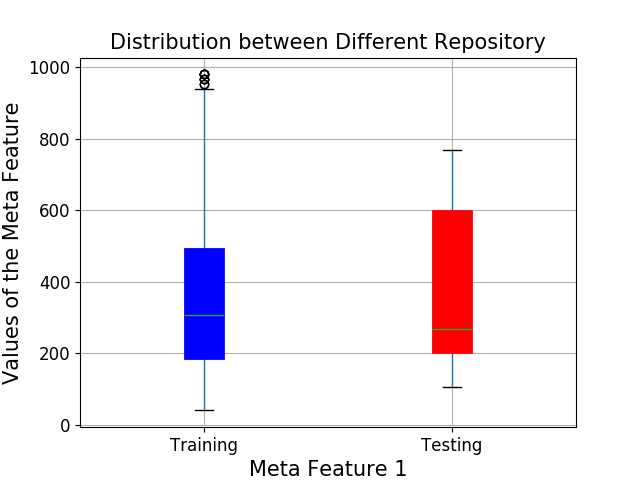
\includegraphics[width=0.8\textwidth]{Figures/Meta_Features/Feature_1.png}
		\parbox{1cm}{\small \hspace{3.5cm}(a){\scriptsize{NS}}}
	\end{minipage}
	\begin{minipage}[t]{0.25\linewidth}
		\centering
		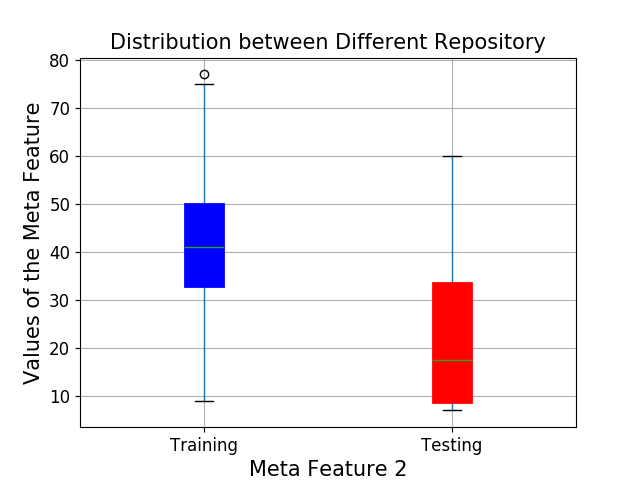
\includegraphics[width=0.8\textwidth]{Figures/Meta_Features/Feature_2.png}
		\parbox{1cm}{\small \hspace{3.5cm}(b)\scriptsize{NF}}
	\end{minipage}
	\begin{minipage}[t]{0.25\linewidth}
		\centering
		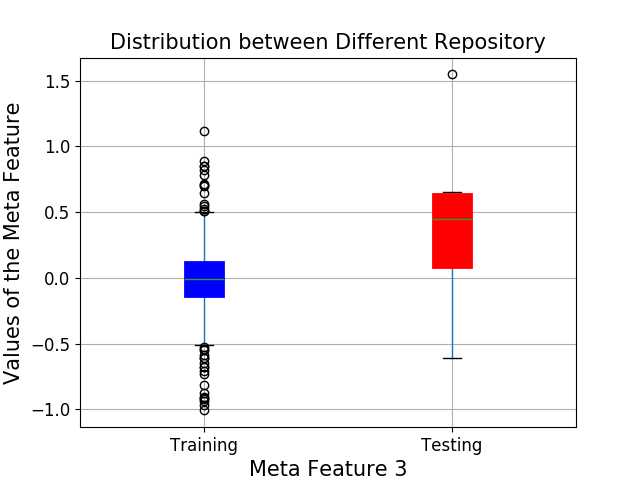
\includegraphics[width=0.8\textwidth]{Figures/Meta_Features/Feature_3.png}
		\parbox{1cm}{\small \hspace{3.5cm}(c)\scriptsize{AAF}}
	\end{minipage}
	\hspace{3ex}
	\begin{minipage}[t]{0.25\linewidth}
		\centering
		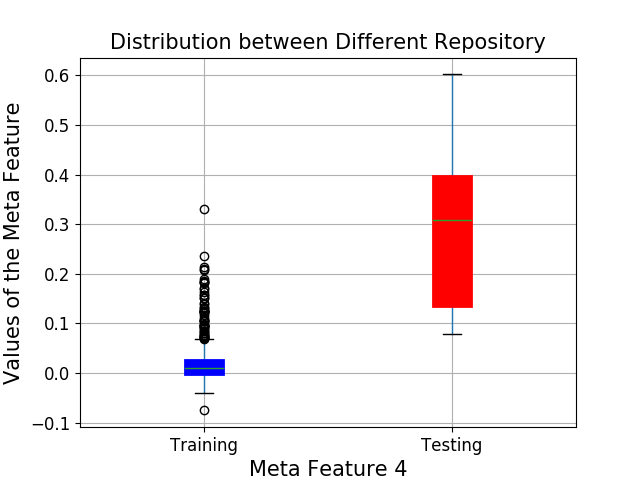
\includegraphics[width=0.8\textwidth]{Figures/Meta_Features/Feature_4.png}
		\parbox{1cm}{\small \hspace{3.5cm}(d)\scriptsize{ACF}}
	\end{minipage}
	\begin{minipage}[t]{0.25\linewidth}
		\centering
		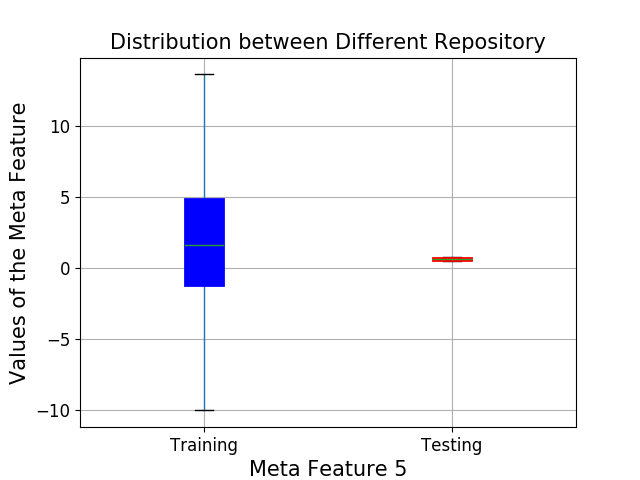
\includegraphics[width=0.8\textwidth]{Figures/Meta_Features/Feature_5.png}
		\parbox{1cm}{\small \hspace{3.5cm}(e)\scriptsize{ACVF}}
	\end{minipage}
	\begin{minipage}[t]{0.25\linewidth}
		\centering
		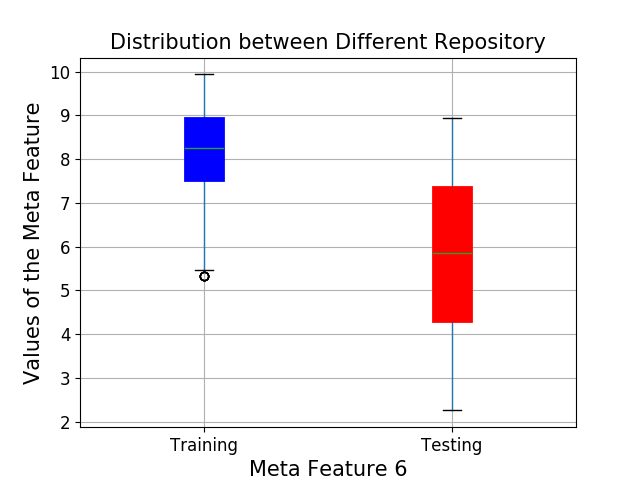
\includegraphics[width=0.8\textwidth]{Figures/Meta_Features/Feature_6.png}
		\parbox{1cm}{\small \hspace{3.5cm}(f)\scriptsize{AEF}}
	\end{minipage}
	\caption{\scriptsize{Comparison of the distribution between the training and testing repository}}
\end{figure}

\begin{itemize}\scriptsize
	\item The distributions in the training repository cover the value range of test datasets well for meta features NS, NF, ACVF;
	\item Meta feature AAF, ACF, AEF of the test datasets are slightly higher or lower than the corresponding value ranges.
\end{itemize}
\end{frame}


\subsection{Evaluation Results}
\begin{frame}
\frametitle{Evaluation Results \UoN}
\begin{columns}
	\begin{column}{0.6\textwidth}
		\begin{table}\tiny
			\centering
			\caption{\scriptsize{Weighted accuracies on 8 test datasets}}
				\begin{tabular}{|c|c|c|c|c|c|c|}
					\hline
					\textbf{Datasets}     & \textbf{GIFS}   & \textbf{ReliefF}     & \textbf{MIFS}  & \textbf{IFS}    & \textbf{\begin{tabular}[c]{@{}c@{}}Best\\ Method\end{tabular}} & \textbf{\begin{tabular}[c]{@{}c@{}}Recommend\\ Method\end{tabular}} \\ \hline
					\textbf{Appendicitis} & \textbf{2.41}  & 2.40   & \textbf{2.41} & 2.40  & G/MIFS  & MIFS  \\ \hline
					\textbf{PIMA}         & $2.63'$  & 2.62  & \textbf{2.64} & 2.56  & MIFS & MIFS          \\ \hline
					\textbf{WBC}          & $3.78'$  & 3.78  & \textbf{3.79} & 3.78  & MIFS & MIFS          \\ \hline
					\textbf{Statlog Heart}  & $4.84'$  & 4.61  & \textbf{4.85} & 4.08  & MIFS   & MIFS      \\ \hline
					\textbf{Parkinsons}   & \textbf{8.52}  & 8.29   & $8.49'$  & 8.42  & GIFS   & ReliefF   \\ \hline
					\textbf{WDBC}         & 13.48    & \textbf{13.60} & $13.51'$    & 13.41  & ReliefF  & ReliefF  \\ \hline
					\textbf{Spectfheart}  & 16.03    & $16.07'$     & 15.85  & \textbf{16.11} & IFS     & MIFS     \\ \hline
					\textbf{Sonar}        & \textbf{16.07} & $15.96'$   & 15.31 & 12.83  & GIFS  & ReliefF         \\ \hline
				\end{tabular}    
		\end{table}
	
	\begin{figure}[tb]
		\centering
		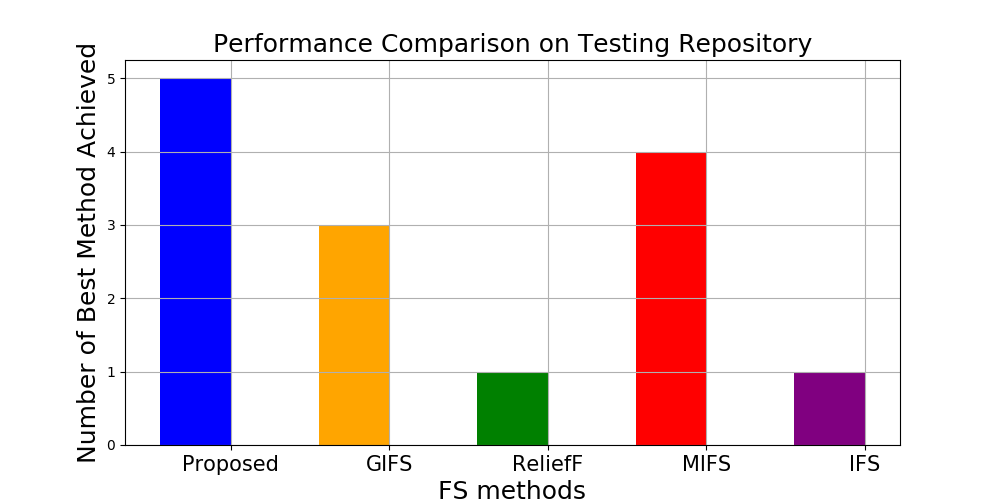
\includegraphics[width=0.6\columnwidth]{Figures/Best_Method_Achieved.png}
		%\decoRule
		\caption{\scriptsize{Performance comparison on testing repository}}
	\end{figure}
	\end{column}
	\begin{column}{0.5\textwidth}
		\begin{itemize}\footnotesize
			\item Successfully recommend best method for Appendicitis, PIMA, WBC, Statlog Heart and WDBC dataset;
			\vspace{0.4cm}
			\item Achieve the best performance comparing with the other individual FS methods;
			\vspace{0.4cm}
			\item Overall, the successful recommendation rate was 62.5\% on the testing repository.
		\end{itemize}
	\end{column}
\end{columns}
\end{frame}


\subsection{Computational Cost}
\begin{frame}
\frametitle{Computational Cost \UoN}
\begin{columns}
	\begin{column}{0.6\textwidth}
		\begin{table}[tb]\scriptsize
			\caption{\scriptsize{Average run time using different methods (/s)}}
			\begin{tabular}{|c|c|c|c|c|c|c|}
				\hline
				\multirow{2}{*}{\textbf{Datasets}} & \multicolumn{4}{c|}{\textbf{Individual Methods}}  & \multirow{2}{*}{\textbf{\begin{tabular}[c]{@{}c@{}}Meta\\Learning\end{tabular}}} & \multirow{2}{*}{\textbf{\begin{tabular}[c]{@{}c@{}}Total Run\\Time\end{tabular}}} \\ \cline{2-5}
				& \textbf{GIFS} & \textbf{ReliefF} & \textbf{MI} & \textbf{IFS} &   &    \\ \hline
				\textbf{Appendicitis}  & 0.37  & 0.36  & 0.32  & 0.09  & 0.07  & 0.39  \\ \hline
				\textbf{PIMA}          & 1.55  & 7.50  & 0.99  & 0.28  & 0.32  & 1.31  \\ \hline
				\textbf{WBC}           & 2.71  & 10.19 & 2.61  & 2.68  & 1.30  & 3.91  \\ \hline
				\textbf{Statlog Heart} & 0.56  & 1.30  & 5.66  & 6.19  & 0.08  & 5.74  \\ \hline
				\textbf{Parkinsons}    & 2.55  & 1.04  & 1.21  & 0.43  & 0.38  & 1.42  \\ \hline
				\textbf{WDBC}          & 15.06 & 6.23  & 3.97  & 1.86  & 2.03  & 8.26  \\ \hline
				\textbf{Spectfheart}   & 3.40  & 3.16  & 4.18  & 2.23  & 0.20  & 4.37  \\ \hline
				\textbf{Sonar}         & 7.66  & 1.74  & 3.36  & 1.29  & 0.72  & 2.46  \\ \hline
			\end{tabular}
		\end{table}
	\end{column}

	\begin{column}{0.4\textwidth}
		\begin{itemize}\small
			\item Meta learning framework takes less than 1 second to run in most cases;
			\vspace{0.4cm}
			\item There is comparatively little additional computational cost incurred in implementing our meta learning framework;
			\vspace{0.4cm}
			\item The use of our meta learning method provides an efficient way to learn the potentially optimal FS method.
		\end{itemize}
	\end{column}
\end{columns}
\end{frame}


\section{Discussion \& Conclusion}
\begin{frame}
\frametitle{Discussion \& Conclusion \UoN}
\begin{block}{Discussion}
	\begin{itemize}
		\item Achieve the best performance comparing with the other individual FS methods;
		\item Introduce very small additional computational burden and be an attractive potential to be used when a wide variety of candidate algorithms are considered;
		\item The results are still provisional and clearly need to be improved in the future.
	\end{itemize}
\end{block}

\begin{block}{Future Work}
	\begin{itemize}
		\item Generate better training data repository with wider distributions, introduce more meta features and test other evaluation metrics for FS;
		\item Use different machine learning methods, various FS methods, datasets with diverse performance, recent meta learning models and etc.
	\end{itemize}
\end{block}
\end{frame}


\begin{frame}
    \begin{figure}
       	\centering
       	
\includegraphics[width=1\columnwidth]{nott_logo/WCCI_Logo.png}
    \end{figure}

    \begin{overpic}[scale=1]{nott_logo/WCCI_Logo.png}
    	\put(15,68){\huge \bf Thank you!}
    	\put(15,65){\huge \bf Questions?}
    \end{overpic}
\end{frame}


\end{document}
